%%   (set-keyboard-coding-system 'utf-8)
\documentclass[tikz]{standalone}
\usepackage{tikz}
\usepackage{pgfplots}
\usetikzlibrary{matrix, positioning, shapes}
\usetikzlibrary{arrows, arrows.meta, automata, shadows, patterns}

\begin{document}
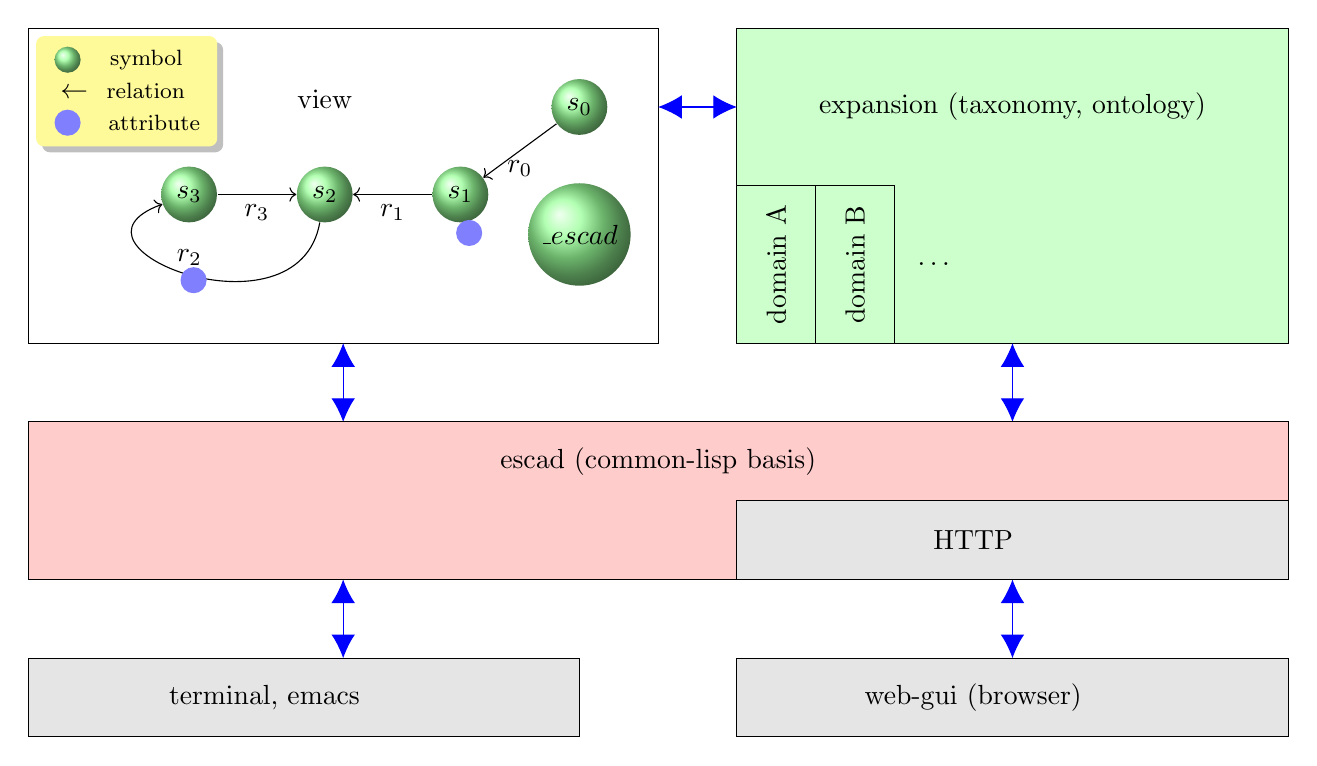
\begin{tikzpicture}[
      node distance=0.6cm and 1cm,
      sym/.style={circle, shading=ball, ball color=green!40, minimum size=0.5mm},
      atr/.style={circle, fill=blue!50, minimum size=0.5mm}]
    \node[sym] (s0) {$s_0$};
    \node[sym] (escad) [below=of s0] {$\_escad$};
    \node[sym] (s1) [below left=of s0] {$s_1$};
    \node[atr] at (-1.4,-1.6) {}; % s1 attribute
    \node[sym] (s2) [left=of s1] {$s_2$};
    \node[sym] (s3) [left=of s2] {$s_3$};
    \draw[->] (s0) -- (s1) node [pos=0.5, below] {$r_0$};
    \draw[->] (s1) -- (s2) node [midway, below] {$r_1$};
    \draw[->,out=-100,in=200,looseness=2] (s2) to node[above,pos=0.5] {$r_2$} (s3);
    \node[atr] at (-4.9,-2.2) {}; % r2 attribute
    \draw[->] (s3) -- (s2) node [pos=0.5, below] {$r_3$};
    \draw[draw=black] (1,1) rectangle ++(-8,-4);
    \node[] (view) [above=of s2] {view};
    %\draw[draw=black, fill=red!20] (2,1) rectangle ++(3,-4);
    %\node[] at (3.5,0) {taxonomy};
    %\node[] at (3.5,-0.5) {(+ontology)};
    \draw[draw=black, fill=green!20] (2,1) rectangle ++(7,-4);
    \node[align=center] at (5.5, 0) {expansion (taxonomy, ontology)};
    \node[] at (4.5,-2) {$\dots$};
    \draw[draw=black] (2,-1) rectangle ++(1,-2) node[rotate=90, pos=.5] {domain A};
    \draw[draw=black] (3,-1) rectangle ++(1,-2) node[rotate=90, pos=.5] {domain B};
    \draw[{Latex[width=3mm, length=3mm]}-{Latex[width=3mm, length=3mm]},blue] (-3,-4) -- (-3,-3) node [pos=0.5] {}; % view - lisp
    \draw[{Latex[width=3mm, length=3mm]}-{Latex[width=3mm, length=3mm]},blue] (5.5,-4) -- (5.5,-3) node [pos=0.5] {}; % expansion - lisp
    %\draw[<->,-{Latex[width=3mm, length=3mm]},blue] (-1,-6) -- (-1,-10) node [pos=0.5] {}; % socket - cli
    \draw[{Latex[width=3mm, length=3mm]}-{Latex[width=3mm, length=3mm]},blue] (-3,-6) -- (-3,-7) node [pos=0.5] {}; % lisp - terminal
    \draw[{Latex[width=3mm, length=3mm]}-{Latex[width=3mm, length=3mm]},blue] (5.5,-6) -- (5.5,-7) node [pos=0.5] {}; % http - web-gui
    \draw[{Latex[width=3mm, length=3mm]}-{Latex[width=3mm, length=3mm]},blue] (1,0) -- (2,0) node [pos=0.5] {}; % view - expansion
    
    \draw[draw=black, fill=red!20] (-7,-4) rectangle ++(16,-2);
    \node[] at (1,-4.5) {escad (common-lisp basis)};
    
    \draw[draw=black, fill=black!10] (2,-5) rectangle ++(7,-1);
    \node[] at (5,-5.5) {HTTP};

    \draw[draw=black, fill=black!10] (2,-7) rectangle ++(7,-1);
    \node[] at (5,-7.5) {web-gui (browser)};
    %\draw[draw=black, fill=black!10] (1,-8) rectangle ++(4,-1);
    %\node[] at (3,-8.5) {REST-API};
    %\draw[draw=black, fill=black!10] (-7,-7) rectangle ++(7,-1);

    \draw[draw=black, fill=black!10] (-7,-7) rectangle ++(7,-1);
    \node[] at (-4,-7.5) {terminal, emacs};
    %\node[] at (3,-10.5) {web-gui (browser)};
    %\node[] at (5.5,-10.5) {$\dots$};
    
    %% legend:
    \draw[draw=none, rounded corners=1mm, fill=yellow!40, drop shadow] (-6.9,0.9) rectangle ++(2.3,-1.4);
    \node[sym] at (-6.5,0.6) {};
    \node at (-5.5,0.6) {\footnotesize{symbol}};
    \node at (-5.8,0.2) {$\leftarrow$\ \ \footnotesize{relation}};
    \node[atr] at (-6.5,-0.2) {};
    \node at (-5.4,-0.2) {\footnotesize{attribute}};
\end{tikzpicture}

\end{document}